\documentclass[dvipdfmx]{article}

\usepackage{amsmath}
\usepackage{graphicx}
\usepackage{titlesec}
\usepackage{tikz}
\usepackage{circuitikz}
\usepackage[T1,T2A]{fontenc}
\usepackage[utf8]{inputenc}
\usepackage[english,russian]{babel}

\titleformat{\section}
            {\normalfont\Large\bfseries}
            {}
            {0pt}
            {Урок \thesection\quad}

\begin{document}

\noindent\makebox[\textwidth]{\rule{\paperwidth}{0.4pt}}
\section{(08.09.2018)}
\noindent\makebox[\textwidth]{\rule{\paperwidth}{0.4pt}}

\subsection{Магнитное поле}

\paragraph{}

Магнитное поле порождается движущимися электрическими зарядами (током).

\paragraph{}

\textbf{Индукция магнитного поля $\vec{B}$} - векторная величина, являющаяся силовой характеристикой магнитного поля.
Определяет, с какой силой поле $\vec{F}$ действует на заряд $q$, движущийся со скоростью $\vec{v}$.

\begin{equation*}
  \vec{F} = q[\vec{v} \times \vec{B}], \quad\quad \vec{B} = [\textup{Тл}]
\end{equation*}
\paragraph{}

Пусть мы переходим из одной системы отсчёта в другую.
Из преобразований Лоренца следует, что:

\begin{equation*}
  F_1 = F_0\sqrt{1-\frac{\upsilon^2}{c^2}},
\end{equation*}
\paragraph{}

где $F_0$ - сила в покое, $\upsilon$ - скорость системы отсчета.

\paragraph{}

Пусть два заряда покоятся. По закону Кулона

\begin{equation*}
  F_0 = \frac{1}{4\pi\varepsilon_0}\frac{q_1q_2}{r^2}
\end{equation*}
\paragraph{}

Перейдем в систему отсчета, движущуюся со скоростью $\upsilon$.\\ Найдем \textbf{обобщенную силу Лоренца}:

\begin{equation*}
  F_1 = \frac{1}{4\pi\varepsilon_0}\frac{q_1q_2}{r^2}
  \frac{\big( \sqrt{1-\frac{\upsilon^2}{c^2}} \big)^2}{\sqrt{1-\frac{\upsilon^2}{c^2}}} =
  \underbrace{\frac{1}{4\pi\varepsilon_0r^2}\frac{q_1q_2}{\sqrt{1-\frac{\upsilon^2}{c^2}}}}_{F_\textup{электр.}} -
  \underbrace{\frac{\upsilon^2}{c^2}\frac{q_1q_2}{\sqrt{1-\frac{\upsilon^2}{c^2}}}}_{F_\textup{магн.}}
\end{equation*}

\paragraph{}

Перепишем формулу для силы магнитного взаимодействия:

\begin{equation*}
  F_M = \frac{\upsilon q_1}{4\pi\varepsilon_0r^2c^2}\frac{\upsilon q_2}{\sqrt{1-\frac{\upsilon^2}{c^2}}}
\end{equation*}
\paragraph{}

Введём индукцию магнитного поля B

\begin{equation*}
  B = \frac{\upsilon q_2}{4\pi\varepsilon_0c^2r^2\sqrt{1-\frac{\upsilon^2}{c^2}}}
\end{equation*}
\paragraph{}
Тогда формула силы магнитного взаимодействия запишется следующим образом:

\begin{equation*}
  F_M = q_1\upsilon B
\end{equation*}
\paragraph{}

Её можно трактовать так: заряд $q_2$ создаёт поле и действует на заряд $q_1$ с силой $F_M$.

\paragraph{}

Для удобства введём константу $\mu_0$:

\begin{equation*}
  \mu_0 = \frac{1}{\varepsilon_0c^2}
\end{equation*}
\paragraph{}

Тогда формула для магнитной индукции

\begin{equation*}
  B = \frac{\mu_0}{4\pi}\frac{\upsilon q}{r^2\sqrt{1-\frac{\upsilon^2}{c^2}}}
\end{equation*}
\paragraph{}

\textbf{Сила Ампера} --- сумма сил Лоренца от нескольких зарядов

\begin{equation*}
  F_A = BIL
\end{equation*}

\newpage

\paragraph{}
Пусть есть бесконечный заряженный провод и заряд $Q$ на расстоянии $x$ от провода. $S$ --- площадь
сечения провода, $\rho$ --- объемная плотность заряда.
\paragraph{}
\noindent\makebox[\textwidth][c]{
\begin{minipage}{0.6\textwidth}
  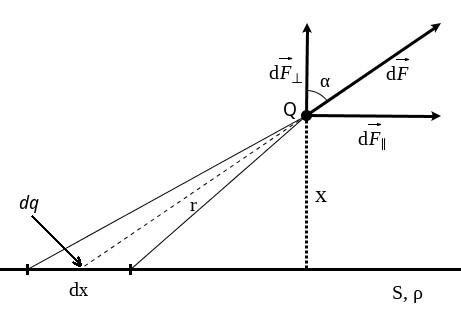
\includegraphics[width=\linewidth,natwidth=461,natheight=316]{images/1.jpg}
\end{minipage}}
\paragraph{}

\begin{equation*}
  dF_\parallel = dFsin\alpha, \quad dF_\perp = dFcos\alpha, \quad dq = \rho Sdx
\end{equation*}

\begin{equation*}
  dF = \frac{1}{4\pi\varepsilon_0}\frac{Q\rho Sdx}{r^2}, \quad r = \frac{x}{cos\alpha},
  \quad dx = \frac{rd\alpha}{cos\alpha}
\end{equation*}

\begin{equation*}
  dF_\perp = \frac{1}{4\pi\varepsilon_0}\frac{Q\rho Sdx}{x^2}cos^2\alpha cos\alpha
\end{equation*}
\paragraph{}

Подставим $r$, $dx$ и проинтегрируем:

\begin{equation*}
  F_\perp = \int_{-\frac{\pi}{2}}^{\frac{\pi}{2}}\frac{1}{4\pi\varepsilon_0}\frac{Q\rho Scos\alpha}{x}d\alpha =
  \frac{Q\rho S}{2\pi\varepsilon_0x}
\end{equation*}
\paragraph{}

Перейдем в систему отсчёта, движущуюся вправо со скоростью $\upsilon$:

\begin{equation*}
  F' = F_0\sqrt{1-\frac{\upsilon^2}{c^2}}, \quad F_M = -\frac{\upsilon^2}{c^2}\frac{Q\rho S}
  {2\pi\varepsilon_0x\sqrt{1-\frac{\upsilon^2}{c^2}}}
\end{equation*}

\newpage

Рассмотрим ток в проводнике с поперечным сечением $S$. Пусть средняя скорость электронов $u$,
$n$ --- объемная концентрация электронов.

\paragraph{}
\noindent\makebox[\textwidth][c]{
  \begin{minipage}{0.6\textwidth}
    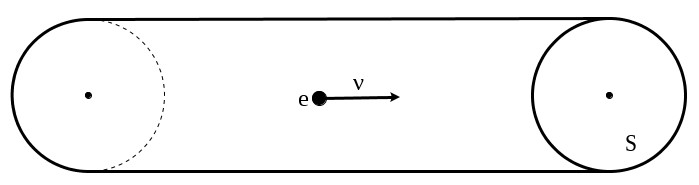
\includegraphics[width=\linewidth,natwidth=699,natheight=185]{images/2.jpg}
\end{minipage}}
\paragraph{}

\begin{equation*}
  I = \frac{\Delta q}{\Delta t} = \frac{enSu\Delta t}{\Delta t} = neSu
\end{equation*}
\paragraph{}

Перепишем формулу $F_M$:

\begin{equation*}
  F_M = -uQ\frac{\mu_0}{2\pi}\frac{\rho S\upsilon}{x\sqrt{1-\frac{\upsilon^2}{c^2}}}
\end{equation*}
\paragraph{}

Но так как $\rho S\upsilon = neS\upsilon = I$, имеем

\begin{equation*}
  F_M = -uQ\frac{\mu_0}{2\pi}\frac{I}{x\sqrt{1-\frac{\upsilon^2}{c^2}}}
\end{equation*}
\paragraph{}

Мы получили формулу \textbf{силы взаимодействия заряда и бесконечного провода.}

\paragraph{}

Рассмотрим теперь случай двух проводников

\noindent\makebox[\linewidth][c]{
\begin{minipage}{0.6\linewidth}
  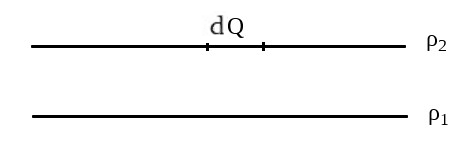
\includegraphics[width=\linewidth,natwidth=473,natheight=157]{images/3.jpg}
\end{minipage}}
\paragraph{}

\begin{equation*}
  dF_M = -\upsilon\frac{\mu_0}{2\pi} \frac{IdQ}{x\sqrt{1-\frac{\upsilon^2}{c^2}}}, \quad dQ = \rho_2Sdx_2,
  \quad dF_M = -\upsilon n_2eS\frac{\mu_0}{2\pi} \frac{I_1dx_2}{x\sqrt{1-\frac{\upsilon^2}{c^2}}}
\end{equation*}
\paragraph{}

Получим формулу \textbf{силы магнитного взаимодействия двух параллельных проводов:}

\begin{equation*}
  dF_M = -\frac{\mu_0}{2\pi} \frac{I_1I_2}{x\sqrt{1-\frac{\upsilon^2}{c^2}}} dx
\end{equation*}
\paragraph{}

Без доказательства примем на веру следующие утверждения:

\begin{equation*}
  \oint_SBds = 0, \quad \oint_lBdl = \mu_0I
\end{equation*}

Второе равенство также называется \textbf{теоремой о циркуляции:} Пусть есть замкнутый ток $I$ и взят некий контур.
Определим \textbf{циркуляцию}, как сумму всех $\vec{B}\cdot d\vec{l}$. Тогда циркуляция в этом контуре равна $\mu_0I$.

\paragraph{}

Магнитное поле является не потенциальным, а вихревым. Это значит, что его силовые линии замкнуты,
а циркуляция отлична от нуля на контуре, который охватывает ток.

\paragraph{}

Рассчитаем магнитное поле, создаваемое бесконечным проводом во всём пространстве:
\paragraph{}
\begin{minipage}{0.4\linewidth}
  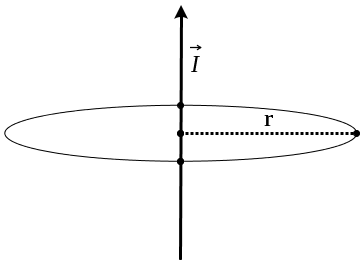
\includegraphics[width=\linewidth,natwidth=364,natheight=266]{images/4.png}
\end{minipage}
\begin{minipage}{0.5\linewidth}
  \begin{equation*}
    B2\pi r = \mu_0I \Rightarrow B = \frac{\mu_0I}{2\pi r}
  \end{equation*}
\end{minipage}

\paragraph{}

Для магнитного поля справедлив принцип суперпозиции: $\vec{B} = \Sigma\vec{B_i}$

\paragraph{Список литературы:}

\begin{itemize}
\item
  Калашников С.Г. Электричество
\item
  Зильберман Г.Е. Электричество и магнетизм
\item
  Сивухин Д.В. Общий курс физики. Т.3. Электричество
\end{itemize}

\subsection{Электромагнитная индукция}
\paragraph{}

В 1831 году Майкл Фарадей провёл следующий опыт:

\paragraph{}
  \noindent\makebox[\linewidth][c]{
  \begin{tikzpicture}
    \draw (0,0)
    to node[draw,circle,fill=white] {A} (0,2)
    to [short] (2,2)
    to [L] (2,0)
    to [short] (0,0);
  \end{tikzpicture}}

Он подключил амперметр к катушке и заметил, что если вводить в неё постоянный магнит, то в цепи появляется ток.
Так было открыто явление \textbf{электромагнитной индукции}.

\paragraph{}

\textbf{Электромагнитная индукция} заключается в том, что переменное магнитное поле
порождает вихревое электрическое. \textbf{Закон Ленца} гласит, что возникающий при этом индукционный ток
направлен в противодействие причинам, его породившим.

\paragraph{}

Определим магнитный поток как произведение магнитной индукции на площадь $S$ и на косинус угла между вектором
$\vec{B}$ и нормалью $n$:

\begin{equation*}
  \Phi = BScos\alpha, \quad
  B = 1 [\text{Тл}], \quad
  \Phi = 1 [\text{Вб}]
\end{equation*}
\begin{equation*}
  \text{ЭДС индукции } \varepsilon_i = -\frac{d\Phi}{dt}
\end{equation*}
\paragraph{}

\noindent\makebox[\linewidth][c]{
\begin{minipage}{0.6\linewidth}
  \textbf{Задача.} Перемычка длины $x$ движется вправо со скоростью $\vec{\upsilon}$.
  \begin{equation*}
    \varepsilon_i = -\frac{\Delta\Phi}{\Delta t} = -\frac{B\Delta S}{\Delta t} =
    -\frac{Bx\upsilon\Delta t}{\Delta t} = -Bx\upsilon
  \end{equation*}
\end{minipage}
\begin{minipage}{0.4\linewidth}
  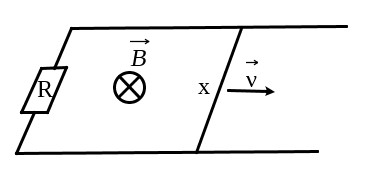
\includegraphics[width=\linewidth,natwidth=368,natheight=181]{images/5.jpg}
\end{minipage}}
\paragraph{}

Тогда возникший индукционный ток будет равен I = $\frac{Bx\upsilon}{R}$ и направлен (по правилу буравчика)
против часовой стрелки.

\begin{equation*}
  \varepsilon_i = IR; \quad \frac{Q}{\Delta t} = \frac{I^2R\Delta t}{\Delta t} = P = \frac{B^2x^2\upsilon^2}{R}
\end{equation*}

\paragraph{Индуктивность катушки.}

Пусть есть катушка. $N$ --- количество витков, $S$ --- площадь сечения.

\begin{equation*}
  \Phi = BSN = \underbrace{\alpha SN}_{L}I
\end{equation*}

\textbf{Индуктивность} $L$ --- коэффициент пропорциональности между электрическим током $I$, текущим в каком-либо
замкнутом контуре, и магнитным потоком $\Phi$.

\begin{equation*}
  L = 1[\text{Гн}]
\end{equation*}

Для соленоида длины $l$ индуктивность равна $L = \frac{l}{b}$, где $b$ --- расстояние между витками. Если же $b = 0$,
то $L = \frac{l}{d}$, где $d$ --- толщина витка.

\begin{equation*}
  \varepsilon_i = -\Phi' = -LI
\end{equation*}

\newpage

\subsection{Движение в электромагнитных полях}

\begin{equation*}
  \vec{F_{\text{Л}}} = \underbrace{q\vec{E}}_{F_\text{ЛЭ}} + \underbrace{q\left[\vec{\upsilon}\times\vec{B}\right]}_{F_\text{ЛМ}}
\end{equation*}
\paragraph{}

Распишем векторное произведение как определитель матрицы:

\begin{equation*}
  \vec{F}_{\text{ЛМ}}
  =
  q
  \begin{vmatrix}
    \vec{i} & \vec{j} & \vec{k}\\
    \upsilon_x & \upsilon_y & \upsilon_z\\
    B_x & B_y & B_z
  \end{vmatrix}
  =
  q\left(
  (\upsilon_yB_z - \upsilon_zB_y)\vec{i}
  +
  (\upsilon_ZB_x - \upsilon_xB_z)\vec{j}
  +
  (\upsilon_xB_y - \upsilon_yB_x)\vec{k}
  \right)
\end{equation*}
\paragraph{}

Получили полезную формулу магнитной составляющей силы Лоренца.

\paragraph{Задача 1.}

Точечный заряд $q$ движется в некоторой плоскости с начальной скоростью $\upsilon$. Вектор магнитной
индукции перпендикулярен плоскости. Определить характеристики траектории движения частицы.

\paragraph{}

\noindent\makebox[\linewidth][c]{
\begin{minipage}{0.6\linewidth}
  Заметим, что $\upsilon = const$, потому что вектор силы Лоренца перпендикулярен $\vec{\upsilon}$, значит
  траектория движения частицы - окружность.
\end{minipage}
\begin{minipage}{0.4\linewidth}
  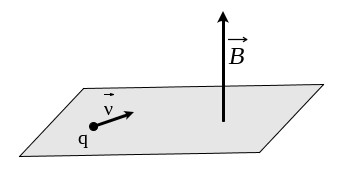
\includegraphics[width=\linewidth,natwidth=342,natheight=188]{images/6.jpg}
\end{minipage}}

Запишем второй закон Ньютона:

\begin{equation*}
  \frac{m\upsilon^2}{R} = q\upsilon B \Rightarrow R = \frac{m\upsilon}{qB}
\end{equation*}

Найдём период обращения $T$:

\begin{equation*}
  T = \frac{2\pi R}{\upsilon} = \frac{2\pi m}{qB}.
\end{equation*}
\paragraph{}

Покажем пример применения полученных результатов:

\paragraph{Задача 2.}

Электрон влетает в однородное магнитное поле ширины $R$. Необходимо определить минимальную скорость,
при которой электрон вылетит из поля.

\paragraph{}

\noindent\makebox[\linewidth][c]{
\begin{minipage}{0.5\linewidth}
  Скорость будет минимальна при такой траектории электрона, что на выходе из поля электрон будет лететь по касательной.
  Так как частица будет лететь по окружности, радиус этой окружности будет равен R.
  \begin{equation*}
    \frac{m\upsilon}{eB} = R \Rightarrow \upsilon = \frac{ReB}{m}.
  \end{equation*}
\end{minipage}
\begin{minipage}{0.5\linewidth}
  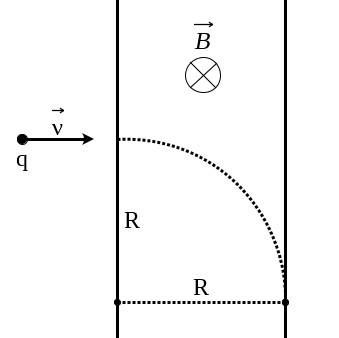
\includegraphics[width=\linewidth,natwidth=358,natheight=309]{images/7.jpg}
\end{minipage}}

\paragraph{Задача 3.}

Точечный заряд имеет произвольный начальный вектор скорости, а вектор $\vec{B}$ перпендикулярен
некоторой плоскости $\gamma$.
Необходимо понять, как будет двигаться заряд.

\noindent\makebox[\linewidth][c]{
\begin{minipage}{0.5\linewidth}
  Вектор $\vec{\upsilon}$ можно разложить на две составляющие: одна лежит в плоскости $\gamma$,
  другая перпендикулярна ей.
  \begin{equation*}
    \vec{F_{\text{Л}}} = q \left[ (\vec{\upsilon}_{\perp} + \vec{\upsilon}_{\parallel})\times\vec{B} \right]
  \end{equation*}
\end{minipage}
\begin{minipage}{0.5\linewidth}
  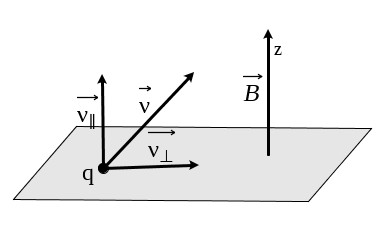
\includegraphics[width=\linewidth,natwidth=383,natheight=230]{images/8.jpg}
\end{minipage}}
\paragraph{}

Если перейти в систему отсчёта, движущуюся вверх со скоростью $\vec{\upsilon}_\parallel$, то в ней траектория частицы
будет окружностью, значит, если вернуться в исходную систему отсчёта, то частица будет двигаться по спирали.

\begin{equation*}
  \upsilon_\parallel = \upsilon cos\alpha, \quad \upsilon_\perp = \upsilon sin\alpha,
  \quad R = \frac{m\upsilon sin\alpha}{qB}, \quad T = \frac{2\pi m}{qB}, \quad h = \frac{2\pi m}{qB} \upsilon cos\alpha
\end{equation*}

\paragraph{Задача 4.}

То же условие, что и в задаче 3, но сонаправленно с $\vec{B}$ действует электрическое поле $\vec{E}$.

\paragraph{}

В этой задаче $\vec{\upsilon_\parallel}$ увеличивается линейно.

\begin{equation*}
  a_z = \frac{qE}{m}, \quad \upsilon_z = \frac{qE}{m}t, \quad z(t) = \frac{qE}{2m}t^2
\end{equation*}

\paragraph{}

\newpage

Рассчитаем расстояние между витками спирали, по которой полетит частица:

\begin{equation*}
  h_n = z_n - z_{n-1} = \frac{qE}{2m}\left(\frac{2\pi m}{qB}\right)^2\left(n^2-(n-1)^2\right) = \frac{2\pi^2Em}{qB}(2n-1)
\end{equation*}

\paragraph{Закон Био-Савара-Лапласа} Вектор магнитной индукции можно определить по формуле:

\begin{equation*}
  B = \int \frac{\mu_0}{4\pi} \frac{ I[\vec{r} \times d \vec{l}] }{r^3} =
  \frac{\mu_0I}{4\pi}\int\frac{[\vec{r}\times d\vec{l}]}{r^3},
\end{equation*}
где $\mu_0 = 4\pi \times 10^{-7}$ Гн/м

\end{document}
